%%%%%%%%%%%%%%%%%%%%%%%%%%%%%%%%%%%%%%%%%%%%%%%%%%%%%%%%%%%%%%%%%%%%%%
% To-do 
% Comentário sobre os valores de parâmetros;
% Breve comparativo com a literatura;
%
%%%%%%%%%%%%%%%%%%%%%%%%%%%%%%%%%%%%%%%%%%%%%%%%%%%%%%%%%%%%%%%%%%%%%%

\documentclass[11pt]{article}

\usepackage{sbc-template}

\usepackage{graphicx,url}

\usepackage[portuguese]{babel}  
\usepackage{amsfonts}
\usepackage[utf8]{inputenc}  
\usepackage[T1]{fontenc}
\usepackage{comment}
\usepackage[round]{natbib} 

\usepackage{etoolbox}
\patchcmd{\thebibliography}
  {\settowidth}
  {\setlength{\itemsep}{0pt plus 0.1pt}\settowidth}
  {}{}
\usepackage[fixlanguage]{babelbib}

\usepackage{mwe}
\usepackage{graphicx}
\usepackage{xcolor}
\usepackage[colorlinks = true,
            linkcolor = blue,
            urlcolor  = blue,
            citecolor = red,
            anchorcolor = blue]{hyperref}
\usepackage[symbol]{footmisc}

\renewcommand{\thefootnote}{\fnsymbol{footnote}}
\selectbiblanguage{brazil}

\sloppy

\title{Quem é Estamira? Uma análise da coerência dos discursos através de combinação de medidas para classificação de texto}{\vspace{-10cm}}


\author{Bruno Aristimunha\inst{1}}


\address{\vspace{-0.15cm}Universidade Federal do ABC -- Santo André -- SP -- Brasil.}

\begin{document} 

\maketitle
\begin{abstract}
This article investigates disorders in natural speech through natural language processing techniques. We analyze the possible incoherent/schizophrenic speech using the Latent Semantic Analysis method and connectivity measures of the co-occurrence graph. Using these measures as attributes, we selected $4$ classifiers to distinguish illogical speech patterns. The chosen \textit{corpus} comes from the lines of characters from the film Estamira (2004), which tells the life of a garbage collector from Rio de Janeiro. This choice is justified by the fact that the narrative is anchored in complex talks of its main character, Estamira, who for long periods conducts obscure dialogues. There is also a discursive clash between the character's lines and the eloquence of her family.
\end{abstract}

\begin{resumo} 
Este artigo investiga os distúrbios no discurso natural através de técnicas de processamento de linguagem natural.  Analisamos o possível discurso incoerente/esquizofrênico através do método de Análise Semântica Latente e de medidas de conectividade do grafo de co-ocorrência. Combinando essas medidas como atributos, empregamos $4$ classificadores para distinguir padrões de fala ilógicos. O \textit{corpus} escolhido é oriundo das falas de personagens do filme Estamira (2004), que conta a vida de uma catadora de lixo do Rio de Janeiro. A escolha da obra justifica-se por uma narrativa ancorada em discursos complexos de sua personagem principal, Estamira, que durante longos períodos conduz diálogos abstrusos. Há, também, choque discursivo entre as falas da personagem e a lógica na eloquência de seus familiares\footnote{Código em: \href{https://github.com/bruAristimunha/estamira-coerencia-discursos}{estamira-coerencia-discursos}, em qualquer interesse escreva: \href{mailto:b.aristimunha@gmail.com}{b.aristimunha@gmail.com} }.
\end{resumo}



\begin{comment}
O discurso incoerente é um sintoma cardinal associado a condições psiquiátricas e neurológicas, e. g., esquizofrenia e bipolar. Essa categoria de distúrbio afeta a comunicação verbal tornando o discurso vago, confuso e ilógico.
\end{comment}
\section{Introdução}

Esquizofrenia é um transtorno psicótico grave de consequência agressiva para os indivíduos. A doença possui alta correlação com situações de vulnerabilidade social e outras patologias neurológicas, como falta de moradia, depressão, ansiedade, \cite{american2013diagnostic}. O espectro da esquizofrenia é diagnosticado pela presença de sintomas como delírios, alucinações, pensamento desorganizado (discurso) e comportamento motor grosseiro. 

O transtorno do neurodesenvolvimento possui sinal claro na linguagem produzida pelo paciente soando extremamente inteligível. Um exemplo de frase inteligível vem do linguista \cite{chomsky1956three} com a frase "ideias verdes incolores dormem furiosamente", que apesar de sintaticamente correta, não apresenta semântica lógica alguma. O diagnóstico prematuro dos sintomas cardinais é de supra necessidade para o tratamento e amenização das fases agudas da psicose. A característica do pensamento desorganizado e incoerência semântica se mostra preditora pelo menos 3 anos antes do primeiro surto psicótico, \cite{bedi2015automated}.

%A esquizofrenia é a 8ª causa de incapacidade em todo mundo \cite{theodoridou2010disease}. Cerca de 5\% a 6\% dos indivíduos com esquizofrenia morrem por suicídio. Em torno de 20\% tentam tirar a própria vida em uma ou mais ocasiões, com alta densidade para indivíduos do sexo masculino jovens, 61\% dos esquizofrênicos apresentam sinais de depressão clínica \cite{gozdzik2011depressive}. 


A grande problemática da avaliação do discurso é que as pessoas que sofrem estresse emocional são incapazes de reconhecer os sintomas, \cite{peralta1998lack}. Para contornar essa problemática e distinguir pacientes com esquizofrenia, nessa pesquisa pretende-se avaliar um espaço de fala de uma pessoa esquizofrênica no filme Estamira. Esse filme é considerando um dos mais fieis com a realidade esquizofrênica, \cite{souza:2008}. A obra retrata de forma semi-estruturada diversos aspectos da vida de Estamira, e possui breves espaços de fala de pessoas com pensamento organizado. Pesquisas anteriores já demonstraram sucesso no reconhecimento de padrões de fala de pessoas esquizofrênicas. Dentre essas pesquisas, podemos citar algumas características importantes no discurso esquizofrênico: alto uso de pronomes de auto-referencialmente e avolia tendendo aos estados negativos, \cite{buck2015differential}. Alguns estudos já colaboram com aplicações de grafos para avaliar conexões de forma automáticas através da fala, \cite{mota2012speech}. Assim, o objetivo desse trabalho é analisar e classificar de forma automática a coerência do discurso na esquizofrenia. Para tanto, devido uma escassez de corpus de pacientes esquizofrênicos selecionamos o filme Estamira.

\section{Fundamentos} \label{sec:fundamentos}

\subsection{Matriz de co-ocorrência}\vspace{-0.1cm}

O texto a ser analisado é representado por uma matriz de co-ocorrência $\mathcal{M}$, em que por linha temos uma palavra única no texto e por coluna temos a ocorrência das $n$ palavras adjacentes. Entendemos como adjacente toda palavra vizinha a essa no texto. Através do $n$ determinamos a profundidade da busca da relação. Quanto maior o nosso $n$, mais semântica será nossa análise, quando menor, mais sintática \cite{daniel:2000}.

\subsection{Análise Semântica Latente}\vspace{-0.1cm}

Análise Semântica Latente - \textit{ASL} consiste em uma abordagem matemática e computacional para descoberta das relações de semelhanças entre textos, excertos ou sentenças dentro de um texto (distribuição semântica). A premissa do método baseia-se em assumir que palavras usadas em contextos similares tendem a ser semanticamente mais semelhantes entre si do que outras.

Com base nessa premissa, dado uma matriz esparsa de co-ocorrência ($\mathcal{M}$), aplicamos o método de decomposição em valores singulares em que obtemos um espaço semântico. Essa decomposição em valores singulares pode ser entendida como: dado uma matriz $\mathcal{M} \in \mathbb{R}^{+}$ com dimensões $i \times j$, fatoremos essa $M$ na forma: $U \cdot \Sigma \cdot V^{*}$, que $U$ é uma matriz unitária ($i \times j$), $\Sigma$ é matriz com valores singulares sobre a diagonal ($i \times j$), e $V^{*}$ sendo a conjugada transposta de $V$, uma matriz unitária do produto entre $U$ e $V^{*}$, que por sua vez produz uma matriz identidade.

Com essa redução induzimos similaridades semânticas da linguagem com base no padrão de uso das palavras em corpus. Através de uma heurística pode-se também descartar as $k$ colunas finais da matriz $U$, e a matriz $\Sigma$ e $V$. A matriz $U$ agora com dimensões $m \times k$ possui uma densidade maior se comparada com a matriz $M$. Esse espaço semântico, dado pela soma dos vetores das palavras individuais, permite medir a quantidade de similaridade semântica.

\subsection{Modelagem por grafo}\vspace{-0.1cm}
Uma outra abordagem possível para analisar diferentes aspectos da linguagem pode ser feita através de modelagem de grafos. Um Grafo $\mathcal{G}$ é definido como um par ordenado $\left \langle \mathcal{V}, \mathcal{E} \right \rangle $, em que $\mathcal{V}$ é conjunto finito e não-vazio de vértices (também conhecido como nós) e $\mathcal{E}$ é o conjunto de arestas (também conhecido como links) dos vértices, $\{\mathcal{E} \subseteq  (u, l) | \{u, l\} \in \mathcal{V}\}$, se $(u, l)$ é uma aresta, logo, os vértices $u$ e $l$ são adjacentes. Desse grafo $\mathcal{G}$, inferimos medidas globais sobre os padrões presentes, para descrever propriedades estatísticas nessa estrutura de dados. Para esse trabalho selecionamos duas medidas para analisar o seu comportamento, sendo elas: coeficiente de agrupamento e comprimento mínimo do caminho

%No contexto de processamento de linguagem natural, teremos que os vértices correspondem as palavras, e cada aresta a uma relação semântica encontrada pela co-ocorrência.

O coeficiente de agrupamento quantifica a influência que um dado vértice $v$ possui para permitir a criação de uma conexão entre os vértices vizinhos. Essa medida pode ser definida como $C_v = \frac{e_{uk}}{d_{v}(d_{v}-1)}$, em $|e_{uk}|$ é o número de dois vizinhos de um vértice $v$ que são conectados entre si, $d_v$ é o grau desse vértice. Computamos a medida em todos vértices e extraímos a média, como: $C(\mathcal{G}) = \frac{1}{N} \sum_{v=1}^{N} C_v$, em que $N = |V|$.  

O comprimento mínimo do caminho pode ser definido como: dado um grafo não direcionado $\mathcal{G}$ com um conjunto de vértices $\mathcal{V}$, com uma função peso tal que $w : \mathcal{E} \to \mathbb{R}$, mapeando as arestas para valores reais. Definimos como peso do caminho do curto $\delta(u, l)$ desde $u$ até $l$ por: $\delta (u, l) = min \{w(p): u \to^{p} l\}$, se há um caminho entre, do contrário $0$. O caminho mais curto será desde vértice $i$ até vértice $j$ e então definido como qualquer caminho $p$ com peso $w (p) = \delta (u, l)$. Para o caminho mais curto para todos os pares de vértice, soma-se tudo e se divide pelo número de pares de vértices ($N \cdot (N - 1)$), ou seja, $L(G) = \frac{1}{N \cdot (N-1)} \sum_{u\neq l} d(v_u, v_l)$. Como o grafo representa um recorte da fala do filme Estamira, usamos essas medidas para quantificar as diferenças estruturais do discurso de Estamira e outros personagens (“não Estamira”). 

\section{Materiais e Métodos}\label{sec:mate}\vspace{-0.15cm}


Reconhecimento do discurso desorganizado geralmente envolve uma análise de como o indivíduo fala em entrevistas semiestruturadas. Como um discurso não coerente pode ser reconhecido facilmente, após um processo de rotulamento é possível a aplicação de algoritmos capazes de reconhecer esse sintoma cardial da esquizofrenia sem entrevistas semiestruturadas.  A Figura \ref{fig:fluxo} ilustra o fluxograma para nossa arquitetura, sendo dividia em cinco etapas: pre-processamento (rotulamento), matriz co-ocorrência, grafo, análise de coerência e classificação.

\begin{figure}[!ht]
    \centering
    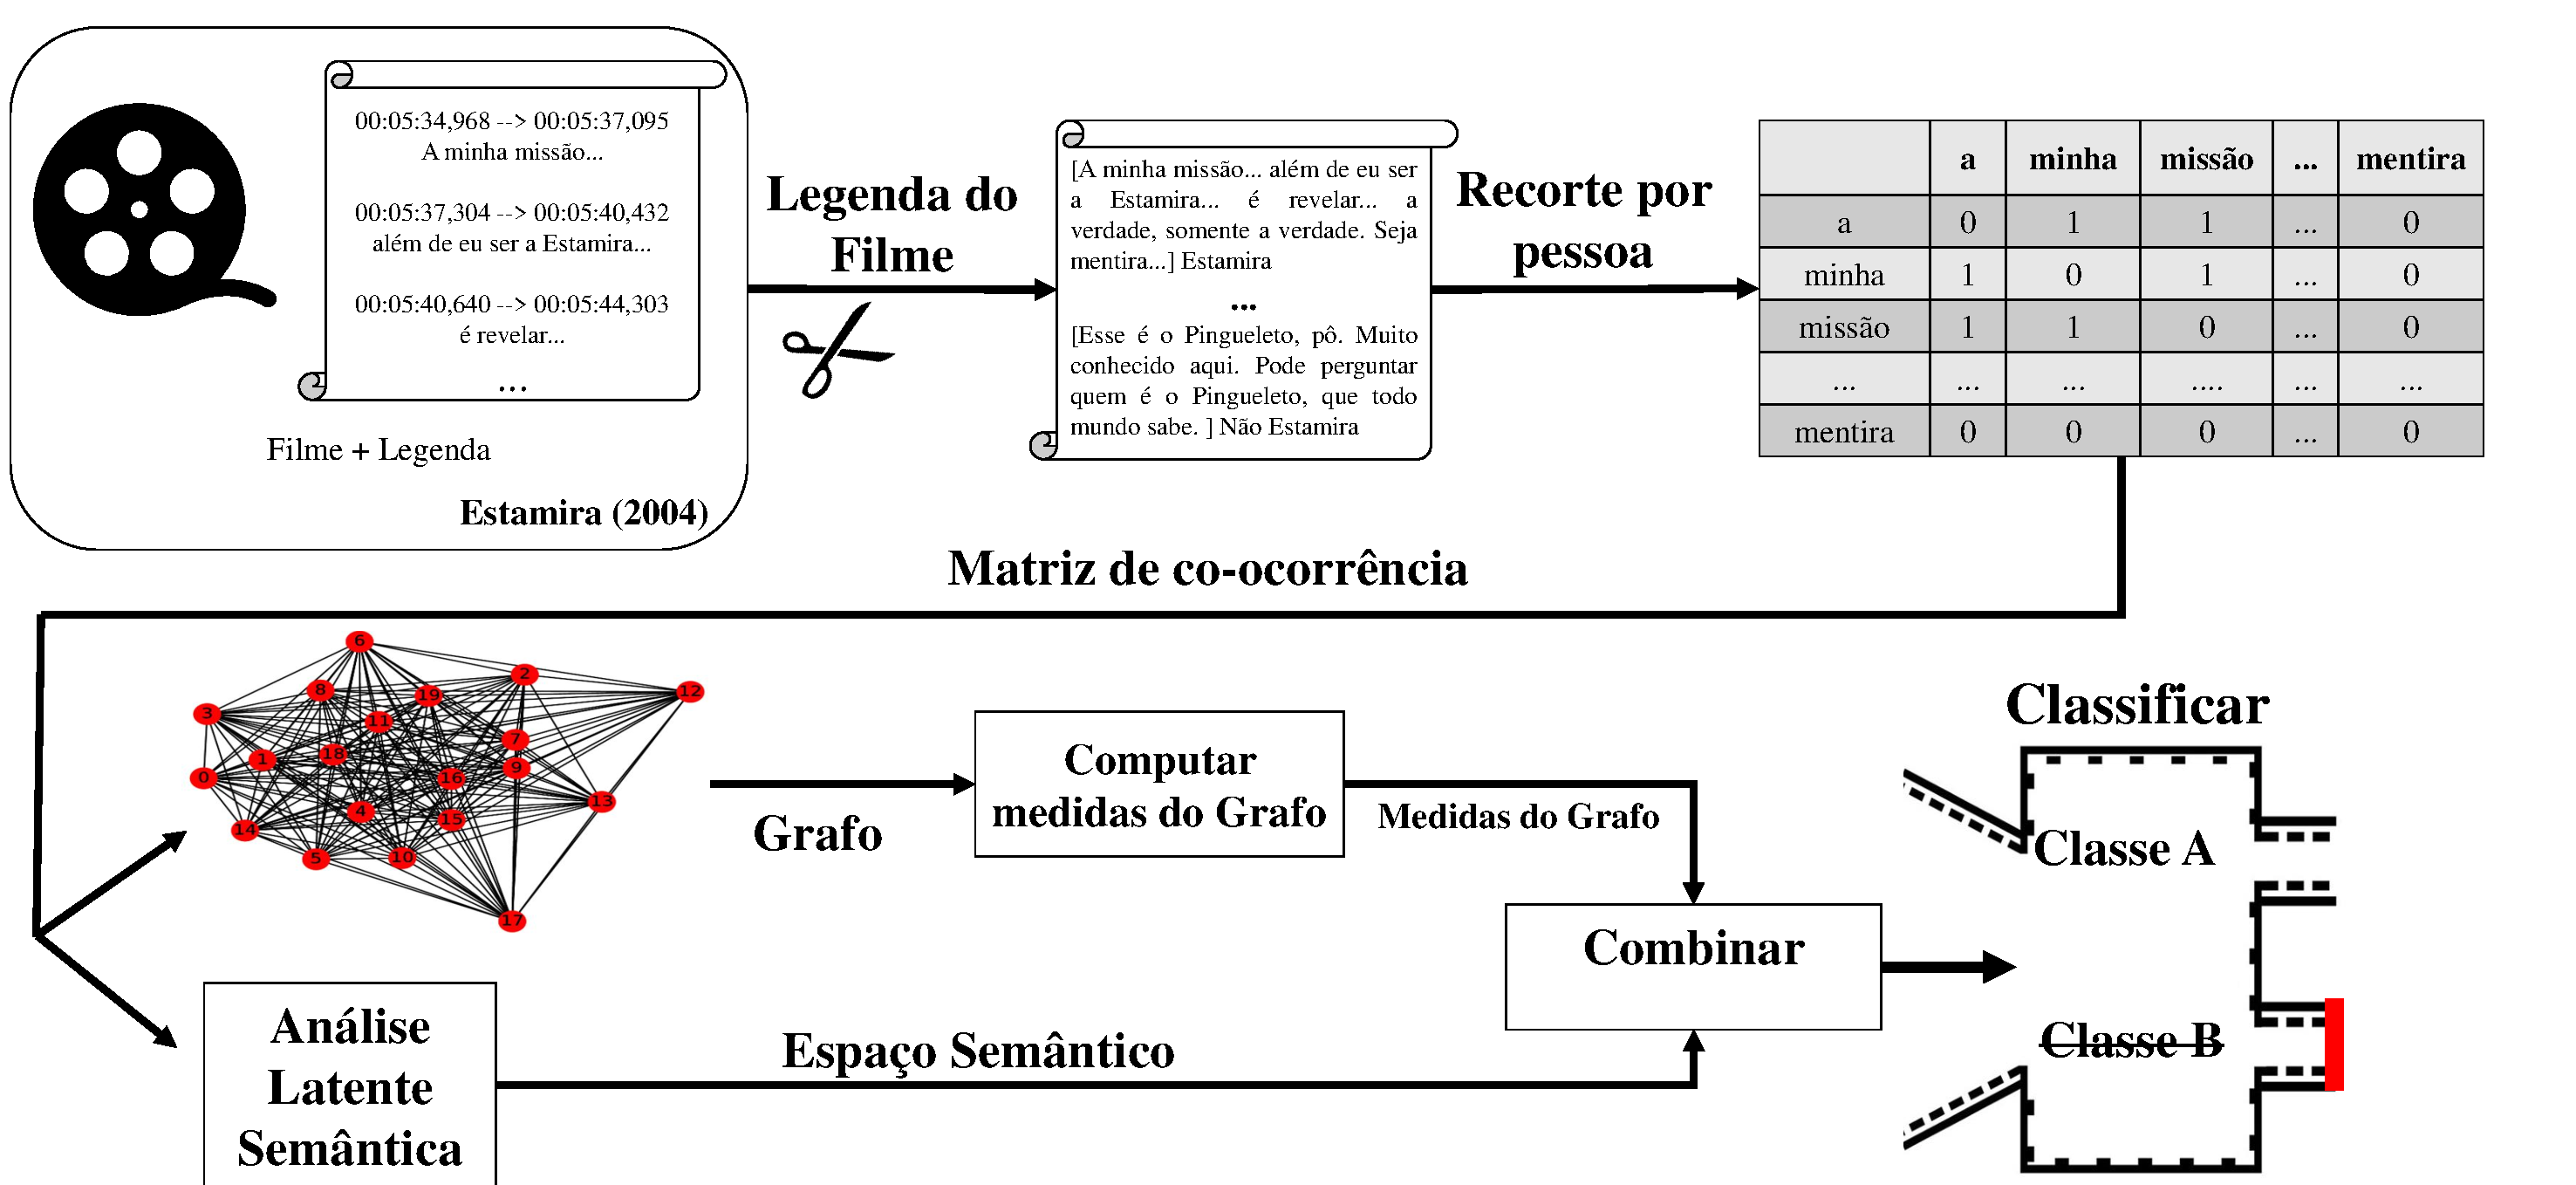
\includegraphics[width=0.8\linewidth]{figures/fluxogramaBruno.pdf}
    \caption{{\footnotesize Cada bloco representa um procedimento e cada seta o fluxo de informação.\vspace{-0.15cm}}}
    \label{fig:fluxo}
\end{figure}


No processo de rotulamento realizamos o recorte das falas de Estamira. Para isso, assistimos o filme, e a cada transição de cena, mudança de assunto ou de personagem, recortamos a fala. No conjunto de falas, rotulamos essas como somente fala da personagem Estamira, e como não pertencente a Estamira (“Não Estamira”). Por fala, geramos uma matriz de co-ocorrência com $n=79$ para análise de Grafo, e também, em paralelo, aplicamos a análise Semântica Latente, sendo o número $79$ corresponde à quantidade media de palavras na frase independente da Classe. Para tarefa do conjunto de dados usado na classificação combinamos as métricas do grafo co-ocorrência, algumas informações sobre as frases, como: a quantidade de caracteres e palavras, e média e desvio padrão do primeiro componente obtido pela análise semântica latente.

Dos algoritmos mais usados na mineração de dados, segundo \cite{top10}, selecionamos os $4$ métodos mais comum na tarefa da classificação: Máquina de Vetor de Suporte (SVM), K-vizinhos (KNN), Classificador Ingênuo Gaussiano e Árvore de Decisão nas características das medidas observadas no grafo e outras informações para predizer de quem é a fala. 

\section{Resultados}\label{sec:resu}

Para avaliar nossa metodologia, calculamos a acurácia ($\mathcal{A}$) dos quatro métodos testados, em validação cruzada com $10$ folhas, com os parâmetros permaneceram com os valores padrões da biblioteca scikit-learn. Na Tabela \ref{tab:acc} podemos observar os resultados de cada método, verificamos que todos os classificadores apresentaram alta variância ($13\% - 34\%$), e resultados medianos, sendo o melhor SVM e o pior o K-Vizinhos.


\begin{table}[!ht]
\centering
\resizebox{0.5\textwidth}{!}{
\begin{tabular}{|c|c|c|}
\hline
Classificador & $\mathcal{A}$ média & $\pm$ \\ \hline
Máquina de Suporte de Vetores & 0.62 & 0.14 \\ \hline
Árvores de Decisão & 0.61 & 0.24 \\ \hline
Naive Bayes Gaussiano & 0.58 & 0.42 \\ \hline
K-Vizinhos & 0.44 & 0.36 \\ \hline
\end{tabular}}
\caption{Média e Incerteza da Acurácia obtida.}%
\label{tab:acc}
\end{table}

Traçando paralelo com os resultados obtidos por \cite{bedi2015automated}, na mesma tarefa, mas com validação \textit{leave-one-out}, nosso resultado se mostra aquém do esperado (100\% de acurácia deles). Isso ocorre, em partes, por conta do ruído no nosso conjunto de dados, e também uma diferença no processo de validação. Já em \cite{Corcoran:2018}, os valores da acurácia variam de 72\% à 83\%, a depender do protocolo. Esses trabalhos dão indícios que os resultados obtidos aqui estabelecem um bom \textit{baseline}, mas que ainda há espaço para melhorias na metodologia.


\section{Conclusão}\label{sec:conc}

O discurso incoerente é um sintoma cardial e complexo para patologias neurológicas, que deve ser analisado e estudado com cuidado médico. Através deste trabalho conseguimos construir uma metodologia, tendo como base um contexto ruidoso de um filme, no qual distinguimos a fala incoerente de Estamira. Como próximo passo, pode-se avaliar a importância do que os classificadores estão aprendendo, visando um melhor entendimento dos padrões do discurso. Pode-se também empregar abordagens distintas para: o recorte da fala, como o reconhecimento por timbre/imagem, e extração de atributos, com modelos de linguagem, \textit{e. g.}, BERT e FastText. Sugere-se também avaliar o contexto da detecção de anomalia, com classificação de uma classe. Propõe-se realizar uma adaptação, em uma próxima etapa, para a inclusão de atributos mais relacionados às características da doença, como contagem de pronomes e análise de sentimentos. 

\section*{Agradecimentos}\label{sec:agr}

Aos professores, pelas sugestões durante a escolha do tema, Walter Hugo Lopez Pinaya; a escolha do \textit{corpus}, Allan Moreira Xavier; a execução, Jesús P. Mena-Chalco. A Matheus Oliveira, pela revisão final do texto.

\bibliographystyle{apalike-ptbr}

{\scriptsize
\bibliography{sbc-template}}

\end{document}
